% This text is proprietary.
% It's a part of presentation made by myself.
% It may not used commercial.
% The noncommercial use such as private and study is free
% Dec 2007
% Author: Sascha Frank
% University Freiburg
% www.informatik.uni-freiburg.de/~frank/
%
%
\documentclass{beamer}
\usepackage{amsfonts}
\usepackage{amssymb,amsmath}
\usepackage{dsfont}
\usepackage{subfigure}


\setbeamertemplate{navigation symbols}{}
\setbeamercolor{frametitle}{fg=black,bg=white}
\setbeamercolor{title}{fg=black,bg=yellow!85!orange}
\usetheme{AnnArbor}
\beamersetuncovermixins{\opaqueness<1>{25}}{\opaqueness<2->{15}}
\DeclareMathOperator*{\argmax}{arg\,max\,}
\DeclareMathOperator*{\minimize}{minimize\,}
\DeclareMathOperator*{\argmin}{arg\,min\,}
\newcommand{\norm}[1]{\left \lVert #1 \right \rVert}
\newcommand{\normtwo}[1]{\left \lVert #1 \right \rVert_2^2}
\newcommand{\normf}[1]{\left \lVert #1 \right \rVert_{Fro}}

\DeclareSymbolFont{letters}{OML}{ztmcm}{m}{it}
\DeclareSymbolFontAlphabet{\mathnormal}{letters}
\SetSymbolFont{letters}{normal}{OML}{ztmcm}{m}{it}
\AtBeginSection[]
{
 \begin{frame}<beamer>
 \frametitle{Plan}
 \tableofcontents[currentsection]
 \end{frame}
}
%%%%%%%%%%%%%%%%%%%%%%%%%%%%%%%55
\begin{document}
\title{Deep Zero-Shot Learning}
\author{Seyed Mohsen Shojaee}
\date{}

\begin{frame}[plain, noframenumbering]
  \begin{center}
\begin{figure}

\includegraphics[scale=0.5]{../images/logo.pdf}
\end{figure}
{\footnotesize Sharif University of Technology \\ Computer Engineering Department \\ MSc Thesis}
\maketitle
\vspace{-10mm}{\footnotesize supervised by \\ Dr.Mahdieh Soleymani} \\
\vspace{4mm}
Summer 2016
\end{center}
\end{frame}



\begin{frame}
  \frametitle{Agenda}
  \tableofcontents
\end{frame}


\section{Introduction}
\begin{frame}
  \frametitle{Introduction}
    \subsection{Standard Learning Paradigm}
    \textbf{Standard Learning Paradigm:}
    Discover the pattern for each class from abundant labeled samples.
    \begin{itemize}
      \item Using SVM, Decision Tree, KNN, etc.
    \end{itemize}
    \begin{figure}
    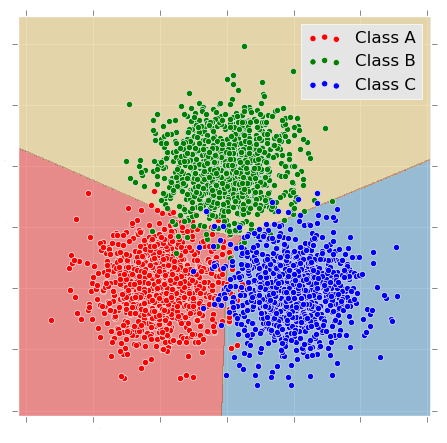
\includegraphics[width= 0.5\linewidth]{multi.png}
    \end{figure}
\end{frame}

\subsection{Zero-shot Learning definition}
\begin{frame}
  \frametitle{Extening the Standard Paradigm}
  Sometimes samples from all classes is not available
  \begin{itemize}
    \item Example: Novel Categories, Fine-grained classification.
  \end{itemize}

  \textbf{Zero-Shot Learning} addresses the problem of classification.
  \begin{itemize}
    \item[]  when no training sample is available for some classes.
  \end{itemize}
  \begin{figure}
  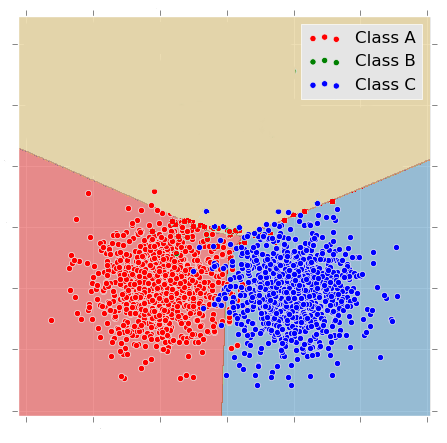
\includegraphics[width= 0.3\linewidth]{zero.png}
  \end{figure}
\end{frame}
\begin{frame}\frametitle{Extening the Standard Paradigm}
\textbf{Identifying Classes without Samples:}
\begin{itemize}
  \item Each category is identified some \textit{auxiliary information} also called
  \textit{signature}.
  \item Examples of class signatures include:
  \begin{itemize}
    \item Attribute Vectors
    \item Text Articles
    \item Category Names
  \end{itemize}
\end{itemize}
\end{frame}
\begin{frame}\frametitle{Extening the Standard Paradigm}
    As a sample, an animal species like Zebra can have these signatures:
    \begin{columns}
    \begin{column}{7cm}
      \begin{itemize}
        \item The Vector (four legs, fast, striped, gallops, non-domestic, ...).
        \item The Wikipedia Entry for zebra.
        \item The word \textit{'Zebra'} itself.
      \end{itemize}
    \end{column}
    \begin{column}{5cm}
      \begin{figure}
      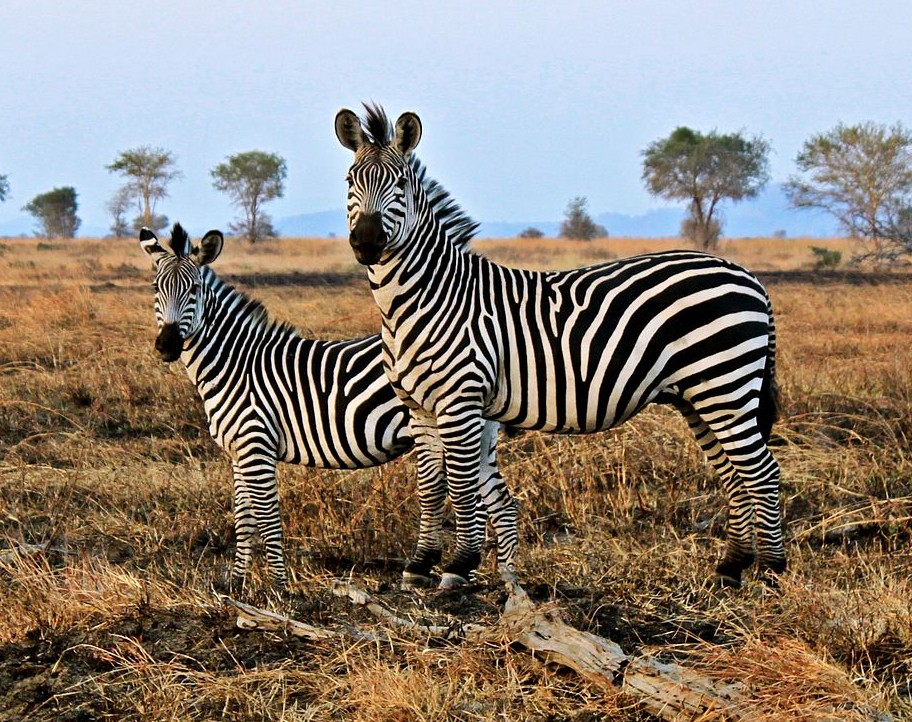
\includegraphics[width= 4cm]{zebra.jpg}
      \end{figure}
    \end{column}
\end{columns}
\end{frame}

\begin{frame}\frametitle{Problem Definition}
  \textbf{At training time:}
\begin{itemize}
  \item there are $N_s$ labeled samples:  $ \{ (\mathbf{x}_i, \mathbf{y}_i) \}_{i=1}^{N_s} $.
  \item These samples are from $n_s$ classes that are called \textit{seen classes}.
  \item Class signatures $C_s$ for seen classes is also available.
  \item There are also $n_u$ classes with no labeled sample. These are called \textit{unseen classes.}
  \item It is assumed in most works that signatures of unseen classes, $C_u$, is also available.
\end{itemize}
\end{frame}

\begin{frame}\frametitle{Problem Definition}
  \textbf{At test time:}
  \begin{itemize}
    \item  $N_u$ samples from unseen classes are presented: $ \{ (\mathbf{x}_i) \}_{i=N_s + 1}^{N_s + N_u} $.
    \item The Goal is to classify test samples into unseen categories.
    \item In other words finding
     $$ \argmin_{\mathbf{y^{\ast}}_i}  \mathbf{y^{\ast}}_i  \neq \mathbf{y}_i, \quad i= N_s +1 , \ldots, N_s + N_u $$
  \end{itemize}
\end{frame}

\subsection{Solution Steps}
\label{sub:Solution Steps}

\begin{frame}\frametitle{Solution Steps}
Most existing solutions for Zero-shot learning consist of these three steps:
\begin{enumerate}
\item Embed images in a semantic space \pause
\item Embed class signatures to same semantic space \pause
\item Assign images to those classes (e.g. using nearest neighbor classifier)
\end{enumerate}
\end{frame}
\section{Prior Works}
\label{sec:Prior Works}
\begin{frame}\frametitle{Prior Works}
  Existing works can be categorized by the semantic space they use:
  \begin{itemize}
    \item Space of signatures (Attribute Prediction).
    \item Space of images.
    \item A third space.
  \end{itemize}
  We review some selected works from each category.
\end{frame}

\subsection{Attribute Prediction}
\begin{frame}\frametitle{Attribute Prediction}
  \begin{itemize}
    \item A large body of work in Zero-shot learning belongs to this category.
    \item The mapping from signature space is considered identity mapping.
    \item Attribute Estimator/Classifier are learned on train images (standard supervised problem).
    \item The Estimator/Classifier is used on test images to find $\mathbf{c}^{\ast}_i$ for image $\mathbf{x}_i$
    \item $\mathbf{x}_i$ is assigned to class with most similar signature:
    $$ \ell(\mathbf{x}_i) = \argmin_{j=n_s+1 \ldots, n_s + n_u} distance(\mathbf{c}^{\ast}_i, \mathbf{c}_j) $$
  \end{itemize}
\end{frame}

\subsection{Mapping to image space}
\begin{frame}
  \frametitle{Mapping to Image Space}
\begin{itemize}
    \item In training time, Learn a mapping from class signatures to image space:
    \[ \phi: \mathbb{R}^{a} \to \mathbb{R}^d \]
    \item This can bee seen predicting linear one-vs-all classifier for each class from its signature.
    \item In test time, classify test images using classifiers predicted from unseen class signatures.
    \item Assign each sample to class whose classifier produces maximum score:
    \begin{equation}
      \ell(\mathbf{x}) = \argmax_{j=n_s+1 \ldots, n_s + n_u} \langle \phi(\mathbf{c}_j), \mathbf{x} \rangle
    \end{equation}
\end{itemize}
\end{frame}

\begin{frame}\frametitle{Semi-supervised Zero-shot Learning}
\end{frame}

\section{Proposed Methods}
\begin{frame}\frametitle{Proposed Methods}
Here we present four proposed methods for the problem of Zero-shot Image Classification.

In our methods we consider class signatures of type attribute vectors.

\begin{itemize}
  \item Attribute Prediction with Multi-task Deep Neural Networks.
  \item Mapping to Histograms of Seen Classes with Deep Neural Network.
  \item Embedding and Clustering
  \item Joint Embedding and Clustering
\end{itemize}
\end{frame}

\subsection{Multi-task Neural Network}
\begin{frame}\frametitle{Multi-task Neural Network}
  We propose a network architecture for attribute prediction from images.

  The network:
\begin{itemize}
  \item  predicts for train and test images at the same time (hence multi-task).
  \item can mitigate the domain shift problem that appears when only samples from seen classes is used.
  \item uses 16 convolutional layers from famous VGG-19 network \cite{vgg}  for feature extraction.
  \item is trained fast using Stochastic gradient descent algorithms family.
\end{itemize}
\end{frame}

\begin{frame}\frametitle{Multi-task Neural Network}
\begin{itemize}
\item[] Let $f$ denote the mapping modeled by the multi-task network.
\item[] Then  $\mathbf{\hat{c}}_i = f (\mathbf{x}_i) $ would be attributes predicted by network for $\mathbf{x}_i$
\item[] We learn $f$ such that:
\end{itemize}
  \begin{equation}
\label{eq:nn_loss}
\minimize_{f}
\frac{1}{N_s} \sum_{i=1}^{N_s} loss(\mathbf{\hat{c}}_i, \mathbf{c}_{y_i}) +
\frac{\gamma}{N_u} \sum_{i=N_s}^{N_s+N_u} \Big ( \min_{j=n_s,\ldots,n_s + n_u} \normtwo{\mathbf{\hat{c}_i - c_j}} \Big ).
\end{equation}
The second term enforces that prediction for test samples to be close to an unseen class signature

Therefore, mitigating domain-shift problem
\end{frame}

\begin{frame}\frametitle{Multi-task Neural Network}
The second term in Eq. \eqref{eq:nn_loss} is modeled by two layers, $q$ and $r$:
\begin{align}
\label{eq:min_layer}
\big(q(\mathbf{v})\big )_j &=  \normtwo{f(\mathbf{v) - c_j}}, \\
r(\mathbf{z}) &= \min_{j=1\ldots n_u} (\mathbf{z})_j.
\end{align}
\begin{itemize}
  \item The $j-$th element of $q$ shows distance of prediction made by network to signature of $j-$th unseen category.
  \item $r$ selects the minimum element of its input
  \item Hence using $q$ and $r$ successively produces distance of prediction to nearest unseen class signature.
  \item This is exactly same as the second term in Eq. \eqref{eq:nn_loss}
\end{itemize}
\end{frame}
\begin{frame}\frametitle{Multi-task Neural Network}
  \begin{figure}
  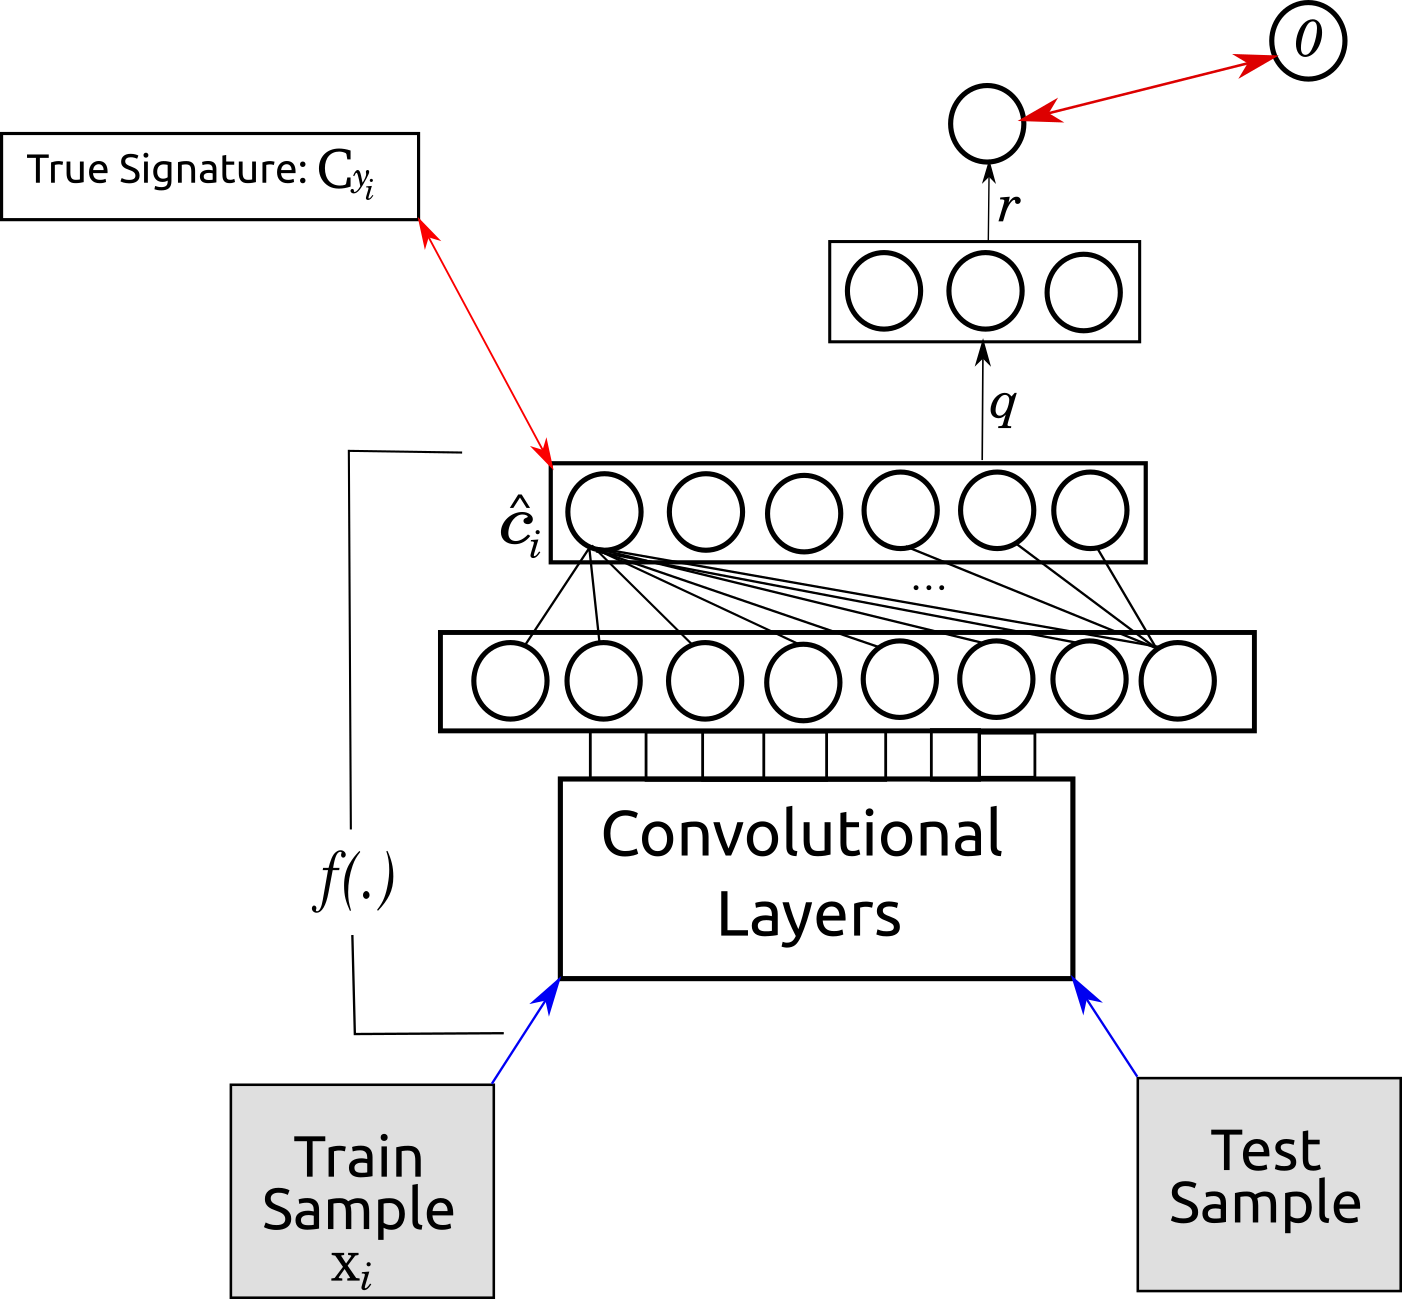
\includegraphics[scale=0.4]{net}
  \caption{Proposed Multi-task network Architecture}
  \end{figure}
\end{frame}

%================================================================================
\subsection{Mapping to Histogram of Seen Classes}
\label{sec:Mapping to Histogram of Seen Classes}
\begin{frame} \frametitle{Mapping to Histogram of Seen Classes}
  \begin{itemize}
    \item
  Motivated by good performance of methods using historgram of similarity to seen
  classes as semantic space \cite{sse}.
\item
  We present a deep neural network that maps images to this space.
  \item
  This network also uses convolutional layers from VGG-19 network.
  \item
  The network is a modification of a typical CNN used in standard supervised classification problems.
\end{itemize}
\end{frame}

\begin{frame} \frametitle{Mapping to Histogram of Seen Classes}
  \begin{itemize}
    \item
  The network  has a standard sequential architecture consisting of 17 pre-trained layers from VGG-19 and four other fully connected layers. \\
  \item
  Size of last layer is equal to the number of seen categories.
  \item
  Let $\phi$ denote the mapping modeled by the network
\end{itemize}
\end{frame}


\begin{frame}\frametitle{Mapping to Histogram of Seen Classes}
  \textbf{In Training Time:}
  \begin{itemize}
  \item Labeled samples from seen classes is used.
  \item Activation function in last layer is softmax:
    \begin{equation}
\label{softmax}
softmax(\mathbf{z})_j = \frac{e^{\mathbf{z}_j}}{\sum_k e^{\mathbf{z}_k}}, \quad j = 1, \ldots, n_s.
\end{equation}
  \item Training criteria is correct label prediction of labeled samples.
  \begin{equation}
  \minimize_{\phi} \sum_{i=1}^{N_s} \sum_{j=1}^{n_s} (\mathbf{y}i)_j \times log(\phi(\mathbf{x}_i)_j) + (1- (\mathbf{y}i)_j) \times log(1 - \phi(\mathbf{x}_i)_j)
\end{equation}
\end{itemize}
\end{frame}

\begin{frame}\frametitle{Mapping to Histogram of Seen Classes}
  \textbf{In Test Time:}
\begin{itemize}
  \item Activation function in last layer is \textit{temprature softmax}:
    \begin{equation}
    \label{softmax}
    softmax_T(\mathbf{z})_j = \frac{e^{\mathbf{z}_j}/T}{\sum_k e^{\mathbf{z}_k}/T}, \quad T>1,  \quad j = 1, \ldots, n_s.
    \end{equation}
\item The softmax layer is trained to produce distribution of true label which is a discrete delta function.
\item When setting $T > 1$ the output becomes smoother.
\end{itemize}
%
\begin{figure}
\hfill
\subfigure[$T=1$]{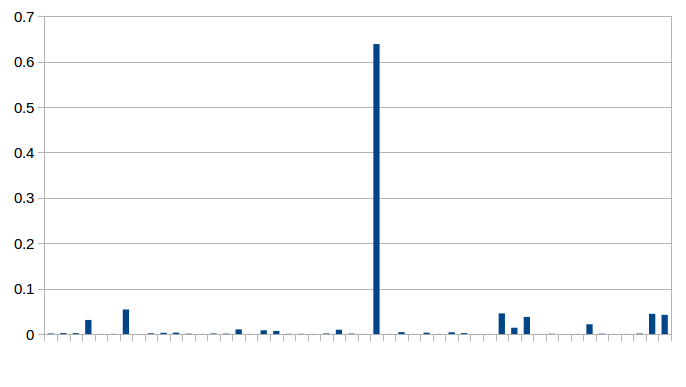
\includegraphics[width=4cm]{softmax}}
\hfill
\subfigure[$T=10$]{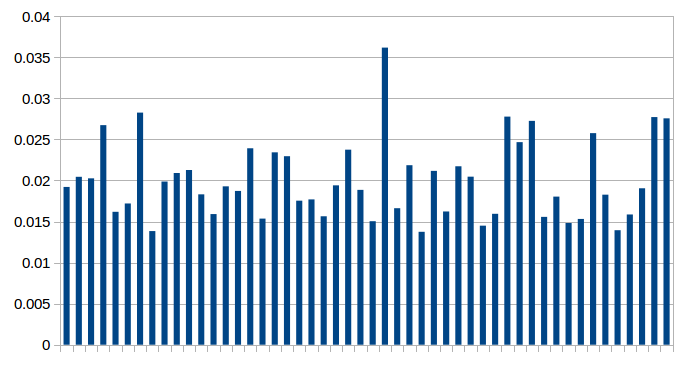
\includegraphics[width=4cm]{tsoftmax}}
\hfill
\end{figure}
\end{frame}

\subsection{Custering and Linear Embedding}
\label{sub:Custering and Linear Embedding}
\begin{frame}\frametitle{Custering and Linear Embedding}
  \textbf{Observation:} 
\end{frame}





\subsection{joining picture and lists}

% \begin{frame}
% \frametitle{pictures and lists in beamer class}
% \begin{columns}
% \begin{column}{5cm}
% \begin{itemize}
% \item<1-> subject 1
% \item<3-> subject 2
% \item<5-> subject 3
% \end{itemize}
% \vspace{3cm}
% \end{column}
% \begin{column}{5cm}
% \begin{overprint}
% \includegraphics<2>{PIC1}
% \includegraphics<4>{PIC2}
% \includegraphics<6>{PIC3}
% \end{overprint}
% \end{column}
% \end{columns}
% \end{frame}


\subsection{pictures which need more space}
\begin{frame}[plain]
% \frametitle{plain, or a way to get more space}
% \begin{figure}
% \includegraphics[scale=0.5]{PIC1}
% \caption{show an example picture}
% \end{figure}
\end{frame}
\begin{frame}[allowframebreaks]
        \frametitle{References}
        {\footnotesize
        \bibliographystyle{apalike}
        \bibliography{references.bib}
        }
\end{frame}
\end{document}
